\documentclass[document.tex]{subfiles}
\begin{document}
\section*{Exercise 1:}

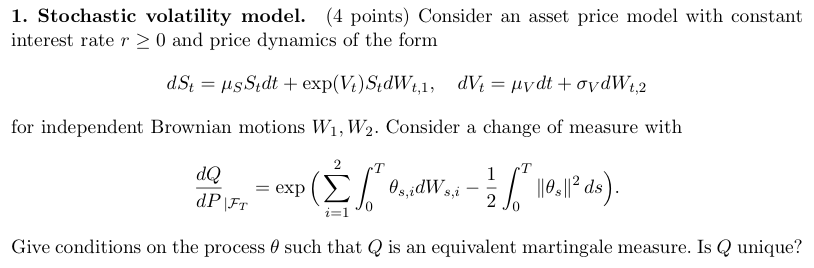
\includegraphics[width=\textwidth]{ex1.png}

For $Q$ being a equivalent martingale measure the discounted asset price process $\tilde{S} = \frac{S}{S^0}$ with \\ 
$S^0 (t) = \int_0^t r_s ds $  has to be a martingale so $\tilde{S_0}= E^Q_0 \lb \tilde{S} \rb$.\\
Conversely 
\begin{itemize}
	\item $\theta$ must be adapted so $\theta_t$ has to be  $\mathcal{F}_t$ measurable for all $t$ \\ 
	\item $P \lb \frac{dQ}{dP} > 0 \rb =1 $
	\item 
	\begin{align*} 
		1 &= E \lb \frac{dQ}{dP} \rb \\
		&= E \lb exp \lb \int_0^t \theta_{s,1} dW_{s,1}+ \int_0^t \theta_{s,2} dW_{s,2} - 
		\frac{1}{2} \int_0^T \sqrt{\theta_{s,1}^2+\theta_{s,2}^2 }ds \rb \rb \\ 
		&= exp \lb -\frac{1}{2} \int_0^T \sqrt{\theta_{s,1}^2+\theta_{s,2}^2 }ds \rb 
		E \lb exp \lb \int_0^t \theta_{s,1} dW_{s,1} \rb \rb 
		E \lb exp \lb \int_0^t \theta_{s,2} dW_{s,2} \rb \rb  
		\end{align*}
\end{itemize}


\end{document}
